\section{แนวคิดและวิธีการดำเนินงาน}

งานวิจัยนี้นำเสนอแนวทางในการสร้างกรณีทดสอบและข้อมูลทดสอบ โดยการรวบรวม{\StaticInformation}ประกอบการพิจารณา 
โดยกรณีทดสอบที่สร้างขึ้นสามารถทดสอบเส้นทางการเรียกหากันอย่างน้อย 1 เส้นทางระหว่างคลาสที่มีปฏิสัมพันธ์กัน 
ซึ่งภาพรวมการดำเนินงานวิจัยนั้นเป็นดังรูปที่ \ref{fig:methodologyoverview} ซึ่งอธิบายได้ดังนี้

\begin{sidewaysfigure}
    \centering
    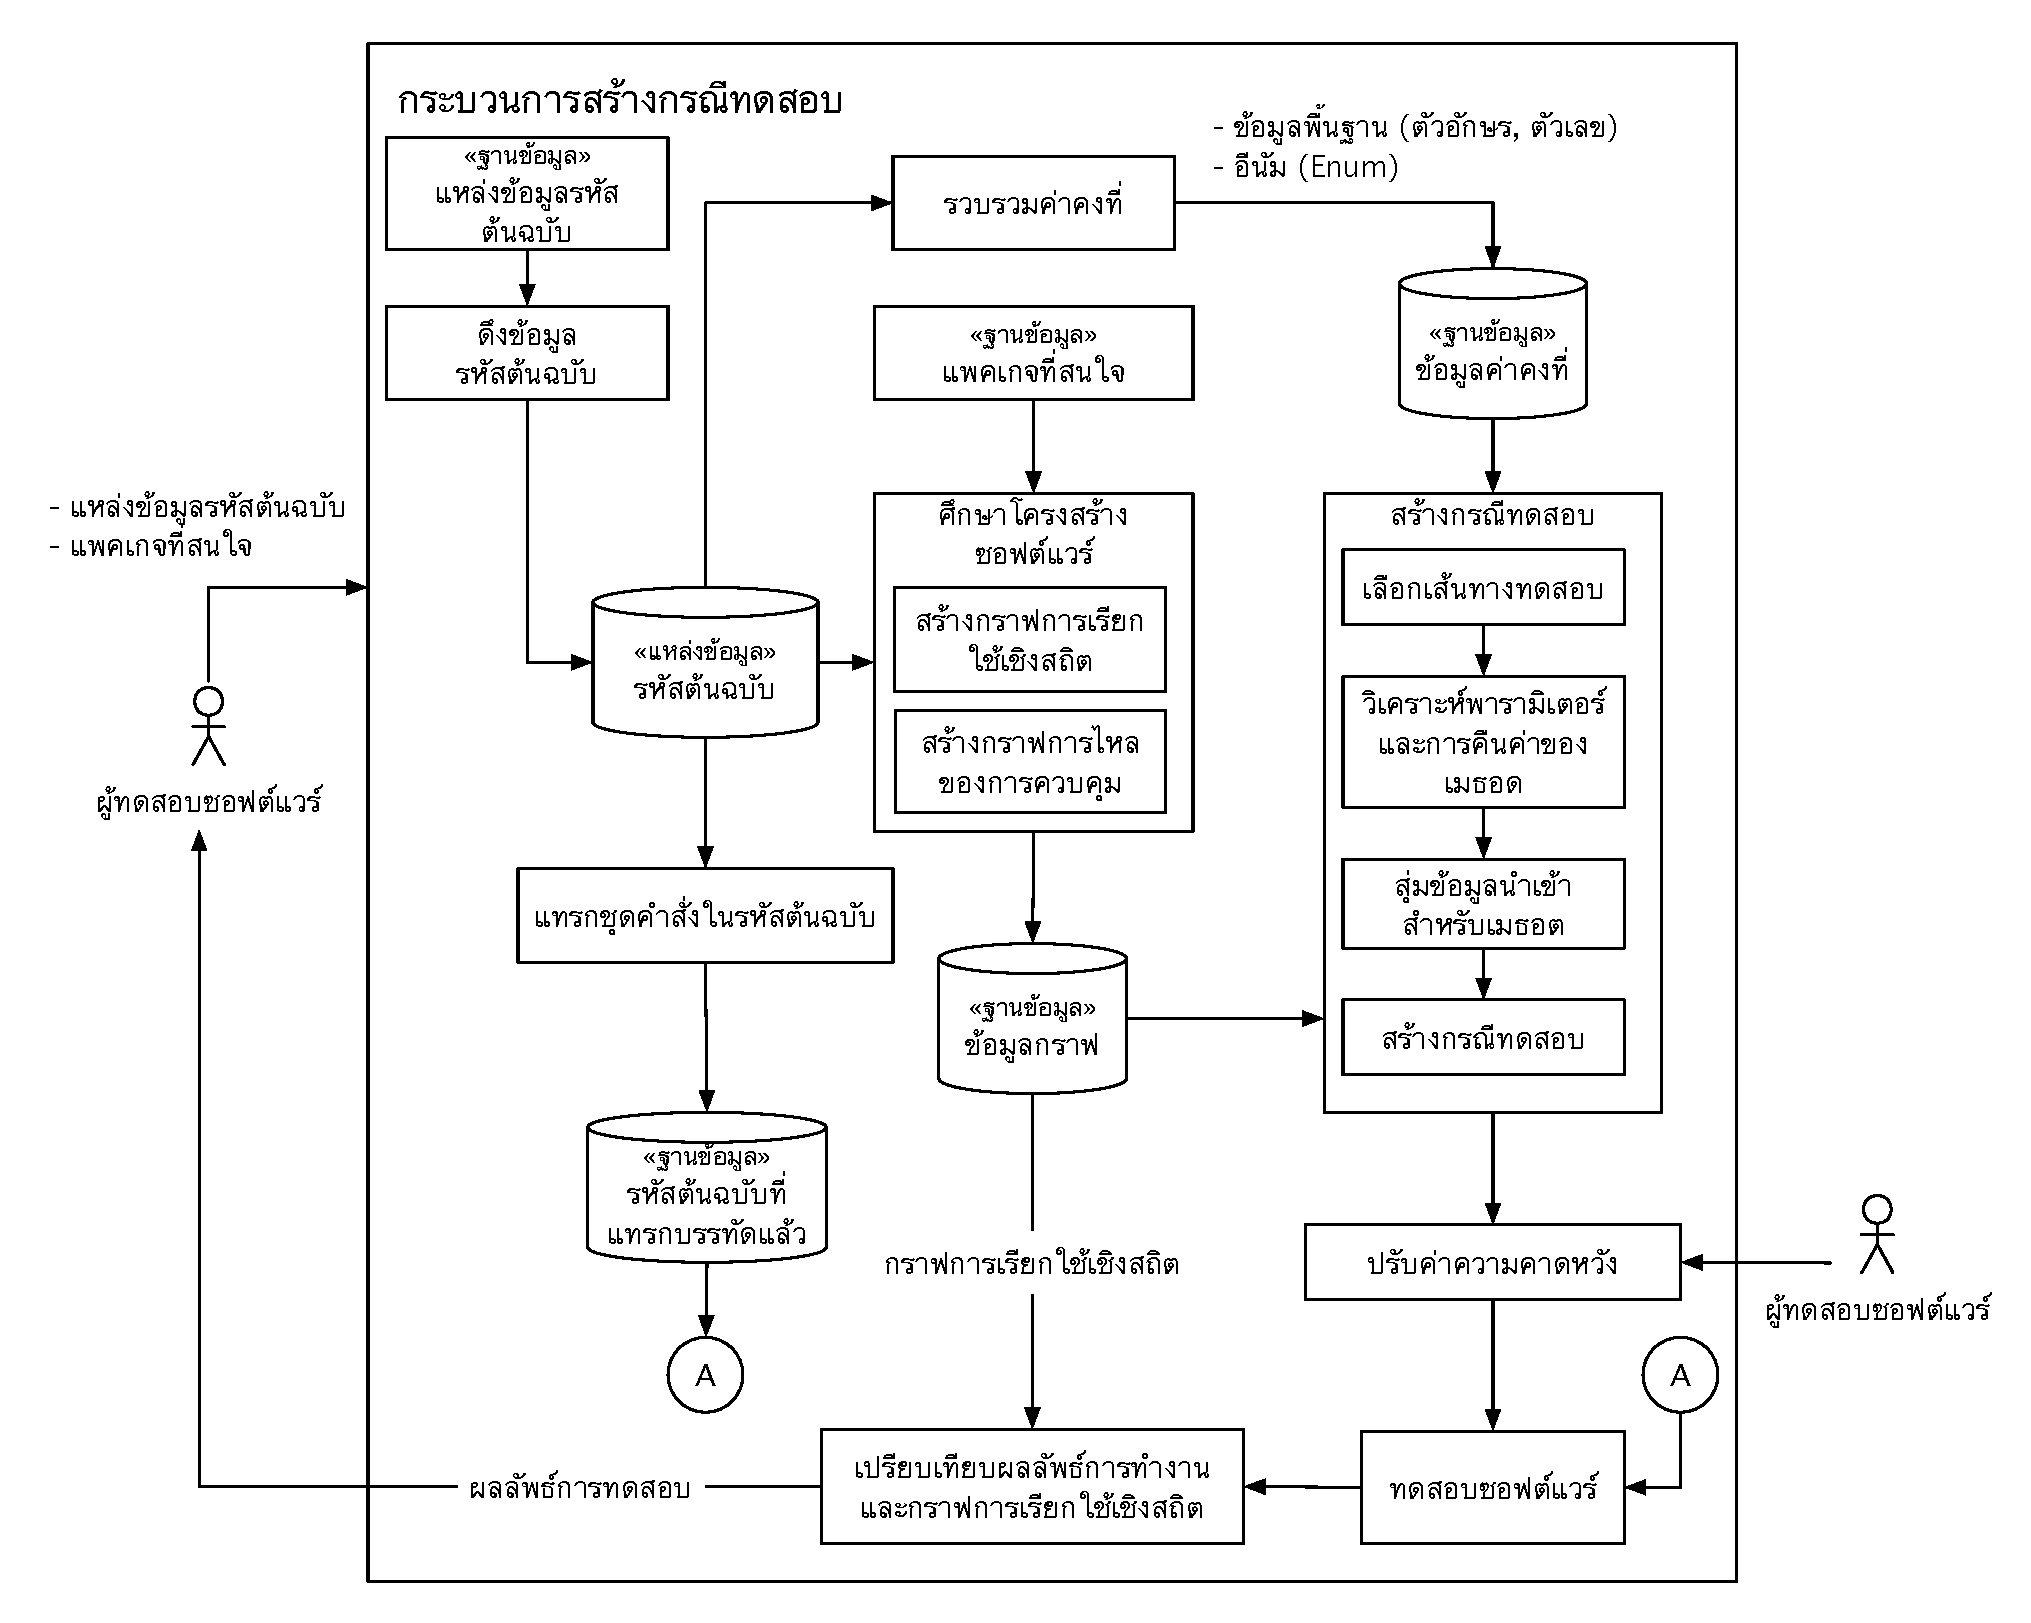
\includegraphics[width=0.9\textwidth]{methodology-overview}
    \caption{ภาพรวมการดำเนินงานวิจัย}
    \label{fig:methodologyoverview}
\end{sidewaysfigure}


\subsection{ภาพรวมงานวิจัย}
% \begin{landscape}
    \begin{sidewaysfigure}
        \centering
        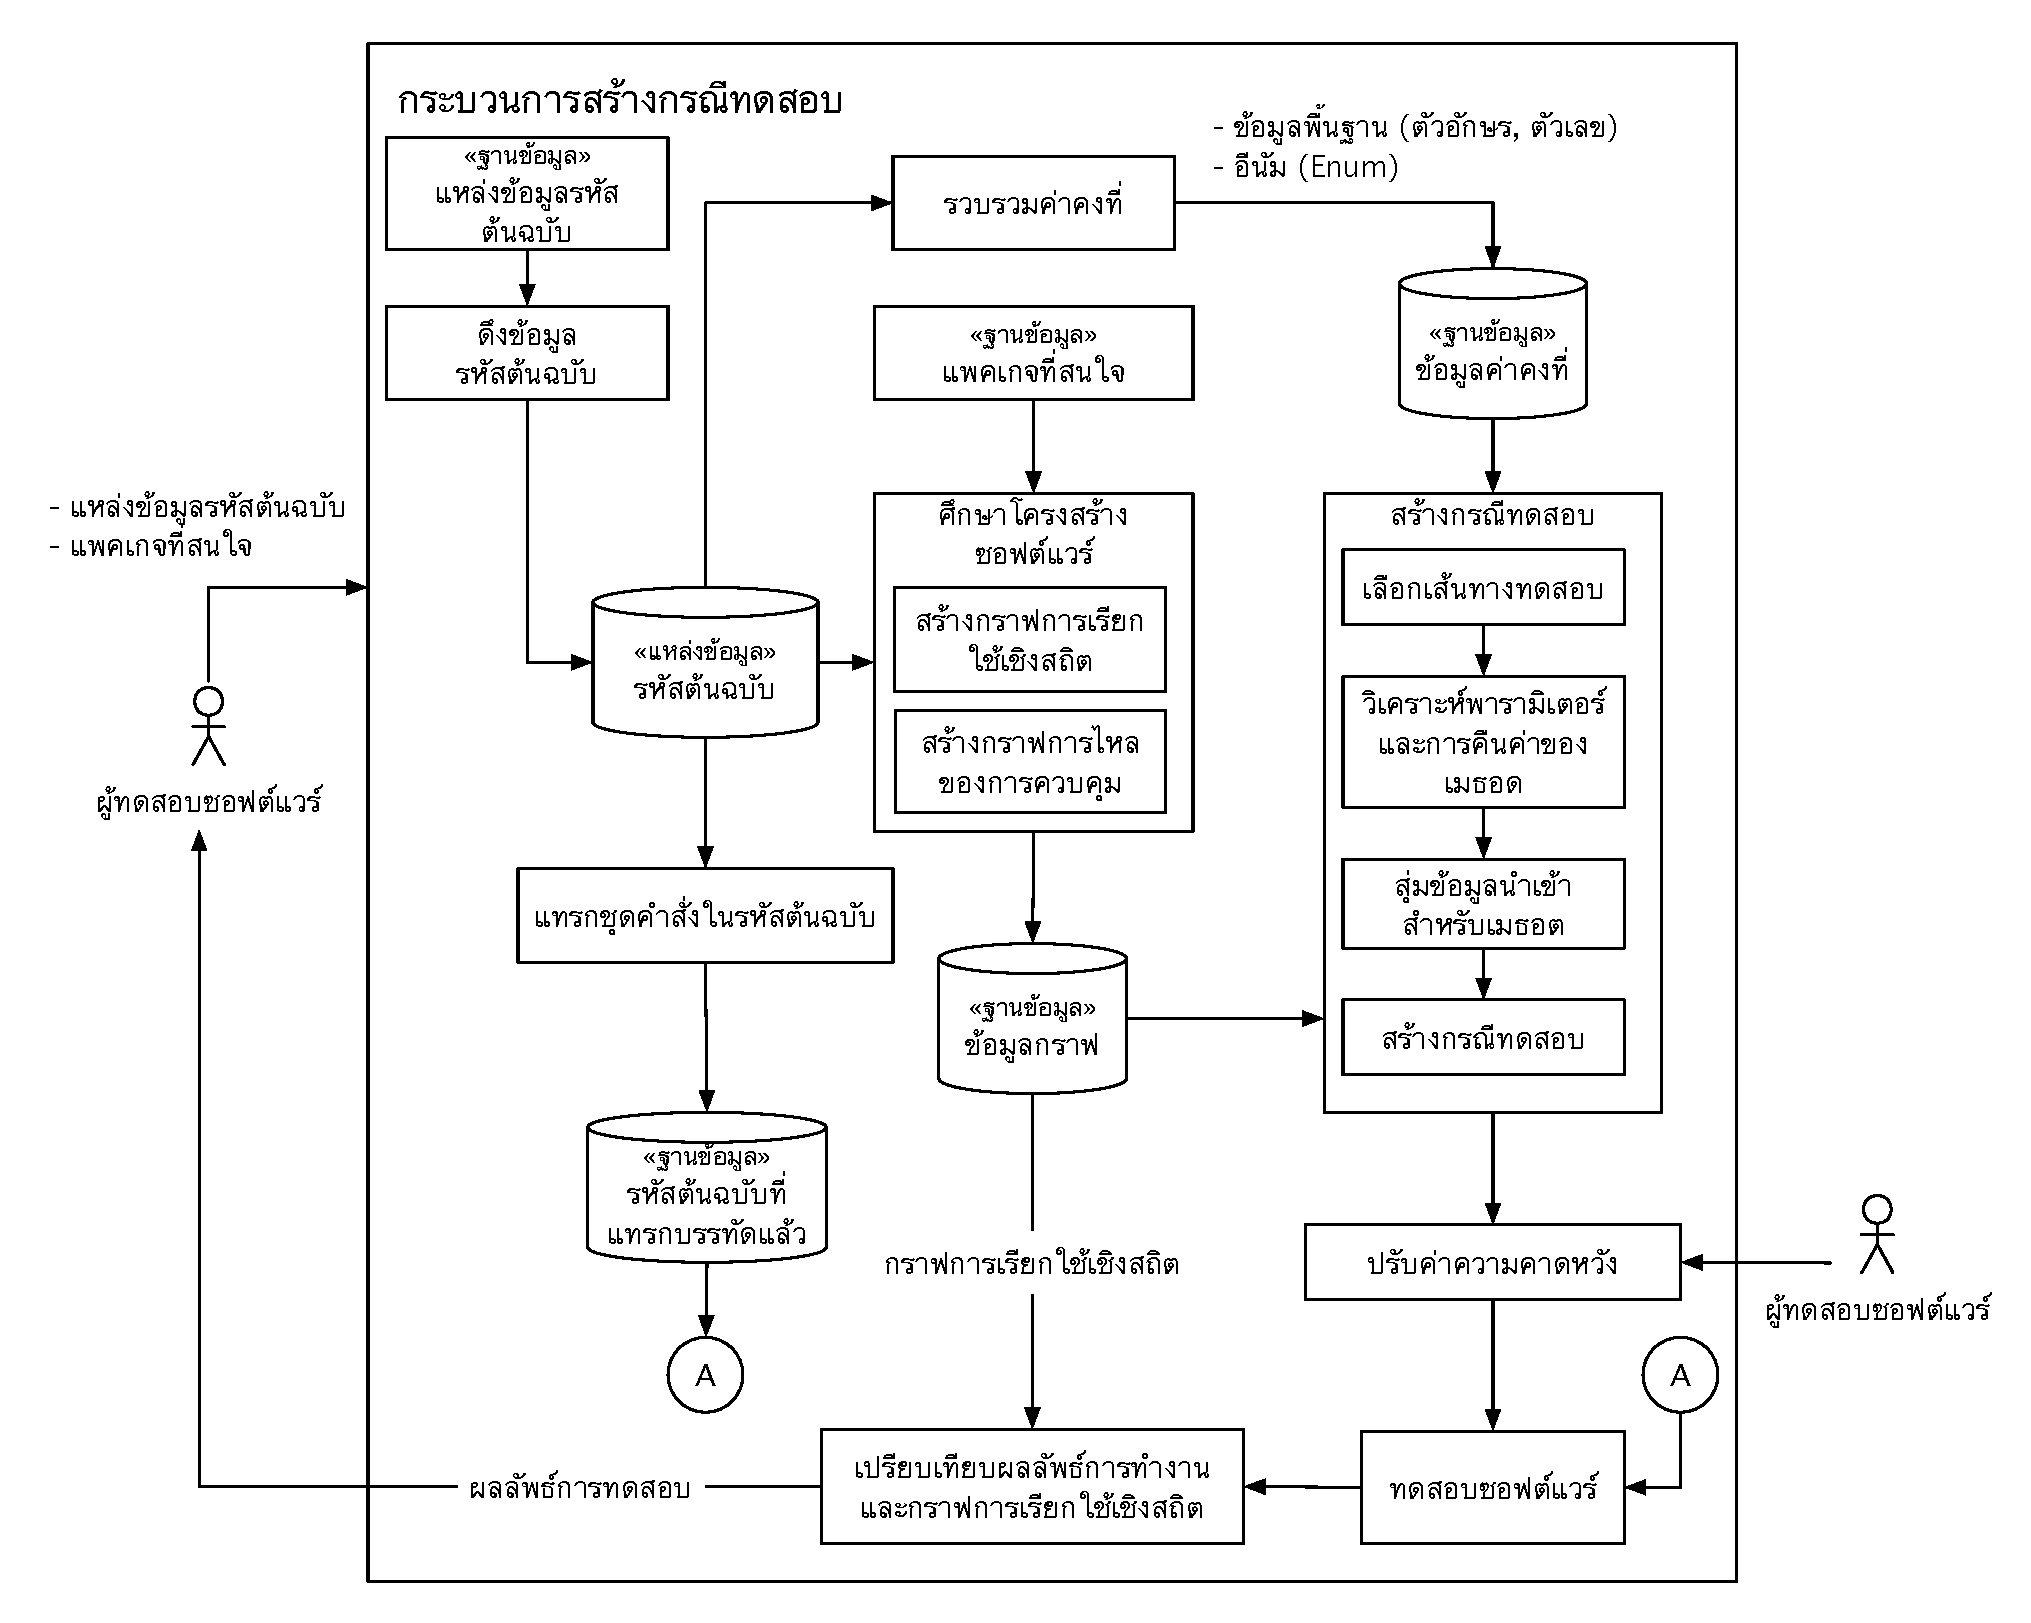
\includegraphics[width=0.9\textwidth]{methodology-overview}
        % 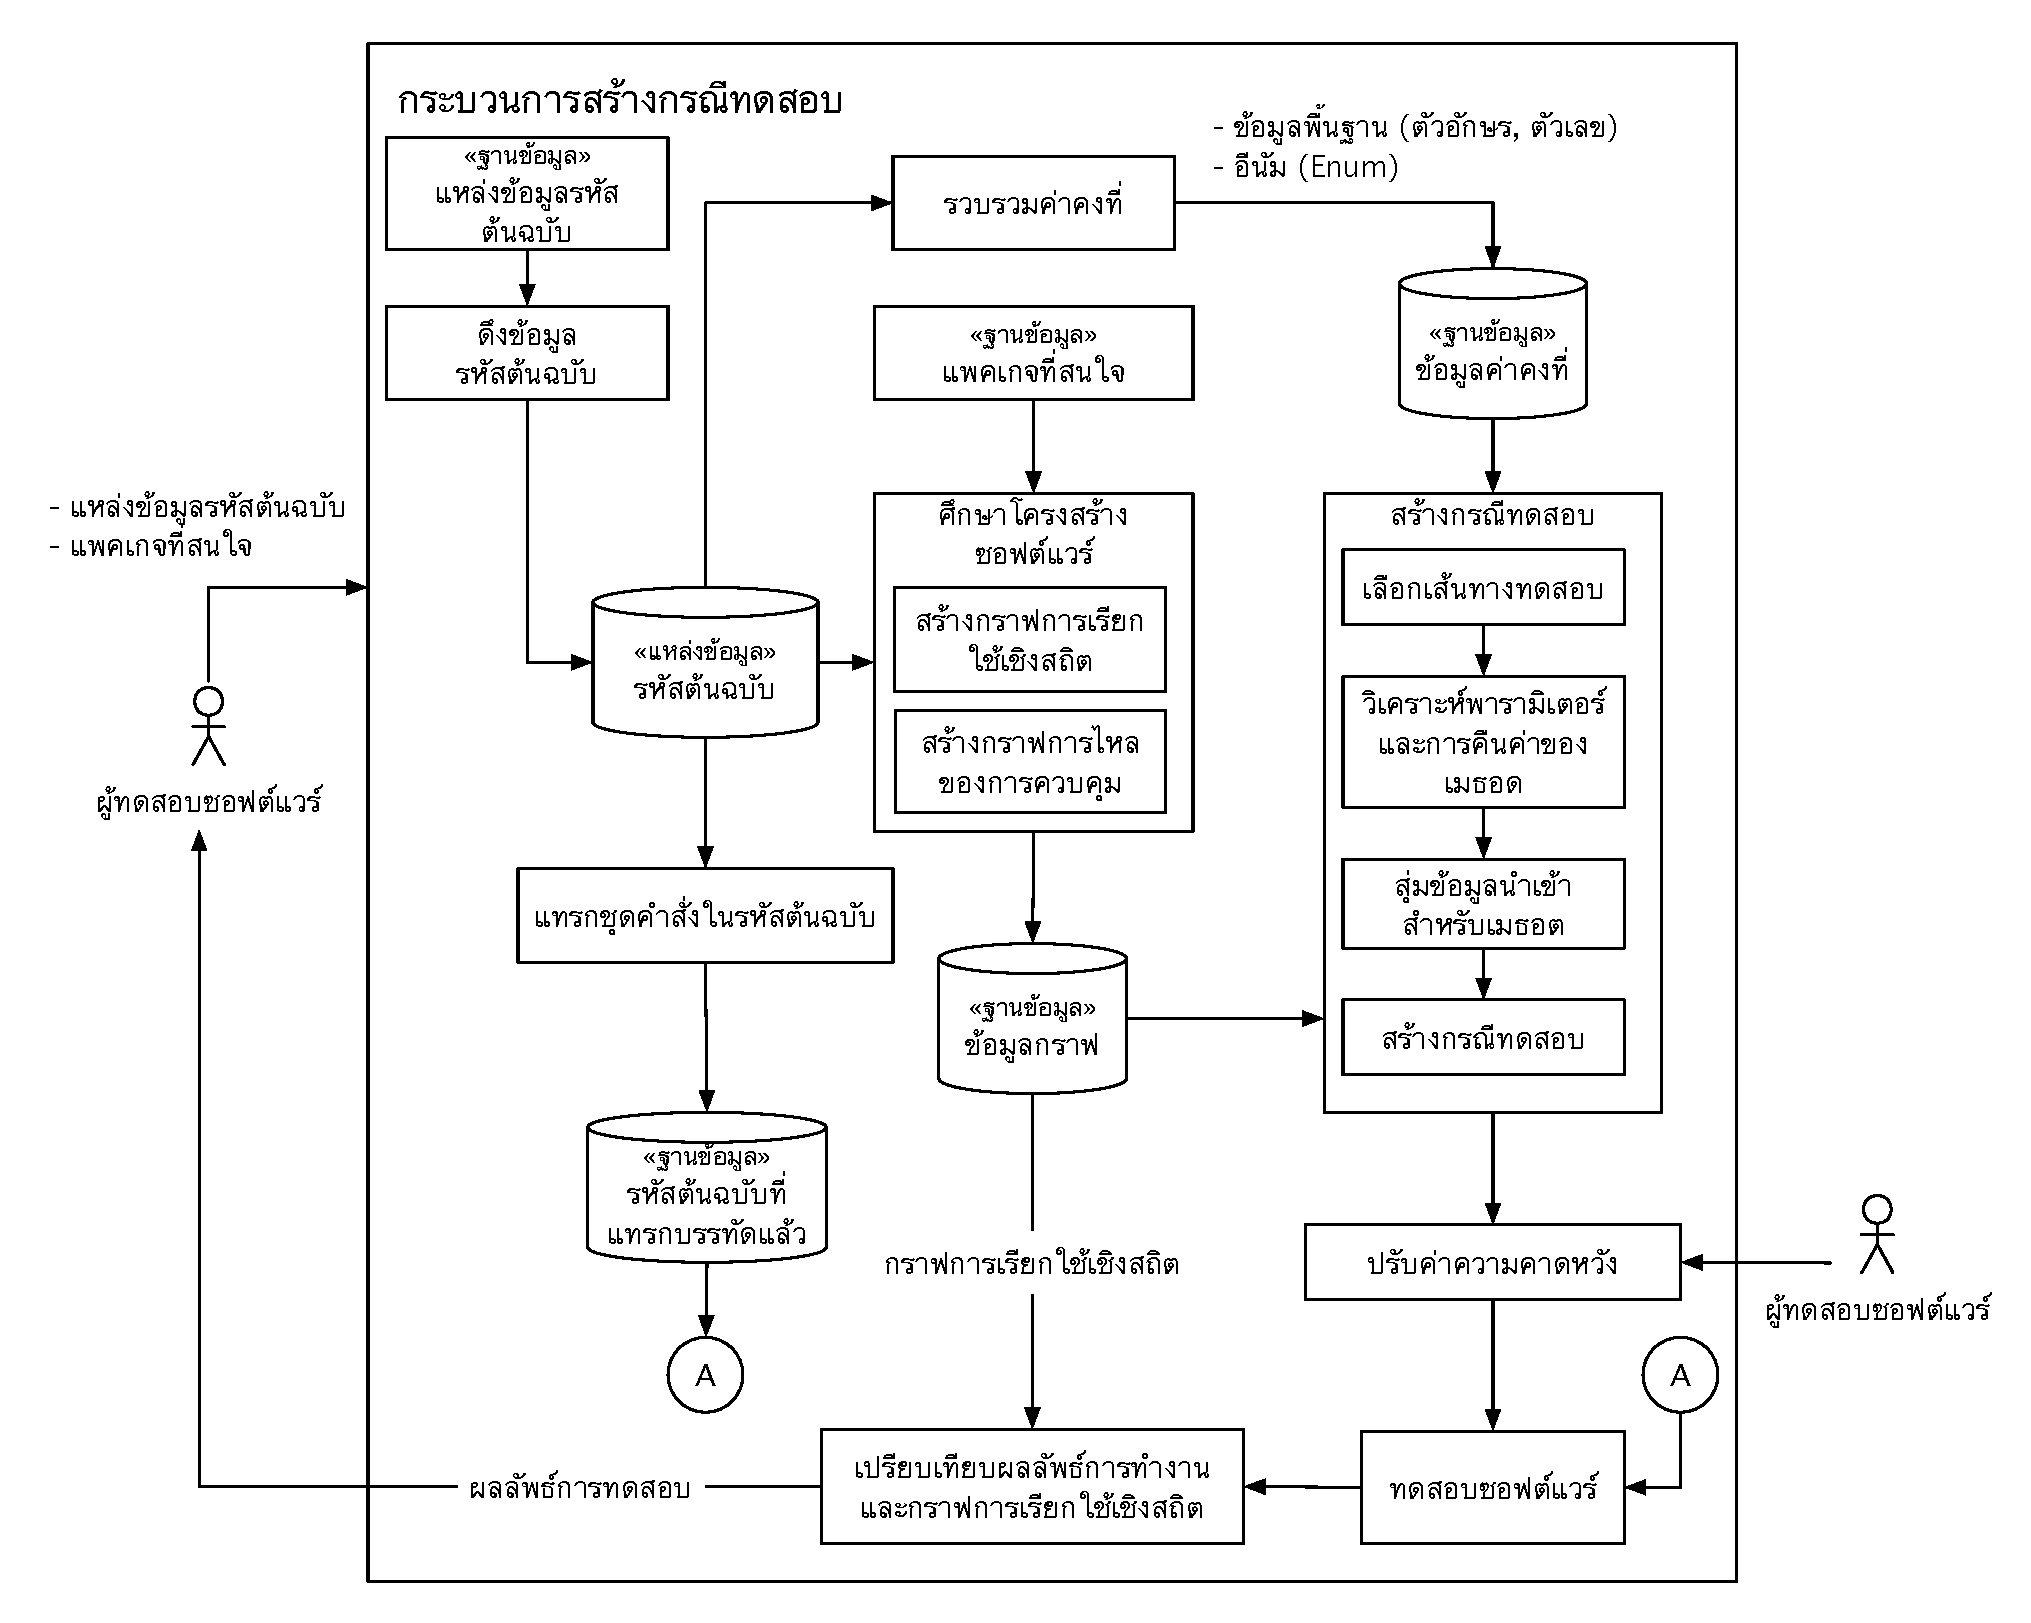
\includegraphics[width=0.9\textwidth]{methodology-overview}
        \caption[setup]{ภาพรวมการดำเนินงานวิจัย}
        \label{fig:methodologyoverview}
    \end{sidewaysfigure}
% \end{landscape}

งานวิจัยนี้นำเสนอแนวทางในการสร้างกรณีทดสอบและข้อมูลทดสอบ โดยการรวบรวม{\StaticInformation}ประกอบการพิจารณา 
โดยกรณีทดสอบที่สร้างขึ้นสามารถทดสอบเส้นทางการเรียกหากันอย่างน้อย 1 เส้นทางระหว่างคลาสที่มีปฏิสัมพันธ์กัน 
ซึ่งภาพรวมการดำเนินงานวิจัยนั้นเป็นดังรูปที่ \ref{fig:methodologyoverview} ซึ่งอธิบายได้ดังนี้

\subsection{การวิเคราะห์ข้อมูลเบื้องต้น}
กระบวนการดำเนินงานนั้นจะเริ่มต้นด้วยการอ่าน{\sourcecode}จาก{\Repository}

\subsubsection{การทำเหมืองข้อมูลค่าคงที่}

\subsubsection{การทำเหมืองข้อมูลค่าคงที่}

\subsubsection{การสร้างแผนภาพ}

\subsection{การสร้างกรณีทดสอบ}

\subsection{การปรับค่าความคาดหวัง}

\subsection{การทดสอบซอฟต์แวร์}

\subsection{เปรียบเทียบผลลัพธ์การดำเนินงาน}

จากรูปที่ \ref{fig:methodologyoverview} การดำเนินงานวิจััยจะเริ่มต้น
